\chapter{ファイルシステム}
ファイルは二次記憶装置(ストレージ)\footnote{
ハードディスク,USBメモリ,メモリカード,CD-ROM,SSD,磁気テープ等の
外部記憶装置(補助記憶装置)のこと.
通常これらは不揮発性であり,電源を切ってもデータが失われることはない.}
に格納された不揮発性のデータ記憶のことである.
通常,一台の二次記憶装置には多数のファイルが記憶される.
ファイルシステムとは,
多数のファイルを二次記憶装置に記憶し管理するために実装された仕組みや,
管理されているファイルの集合のことである.

ここでは,UNIXファイルシステムを例に,
ユーザから見たファイルシステムの構造や仕組みを紹介する.
WindowsやmacOS\footnote{macOSはUNIXの一種と考えてもよい.
}等のファイルシステムも,
基本的な考え方はUNIXと共通である.

%----------------------------------------------------------------------------
\section{ファイル木}
\figref{filesystem}にユーザから見たUNIXファイルシステムの構造を示す.
ファイルはディレクトリ(フォルダ)により階層的に管理されている.
ディレクトリとファイルからなる\figref{filesystem}のような構造を
ファイル木(ファイルツリー)と呼ぶ.

\begin{myfig}{btp}{ユーザから見たUNIXファイルシステムの構造}{filesystem}
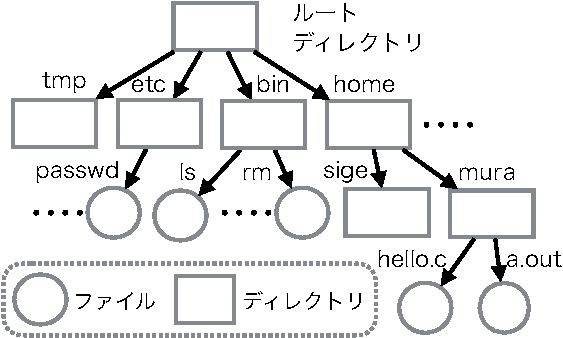
\includegraphics[scale=1.0]{Fig/FileSystem-crop.pdf}
\end{myfig}

ファイル木はルートディレクトリを根(ルート)とする有向の木構造\footnote{
グラフ理論の木構造と似ているが閉路を許す場合もある.}である.
木構造の節点(ノード)はディレクトリであり,葉(リーフ)はファイルである.
有向枝(エッジ)はリンクとも呼ばれる.
リンクには必ず名前が付けられている.
\emph{ファイルの本体とリンクは独立している.}
なお,UNIXファイルシステムではディレクトリもファイルの一種と考える.

%----------------------------------------------------------------------------
\section{特別なディレクトリ}
\figref{filesystem2}に特別なディレクトリを意識して書き直した
ファイル木の一部を示す.
細部にこだわって描いた\figref{filesystem2}は木構造と呼ぶには相応しくないが,
UNIXファイルシステムの実装をより忠実に表現している.

\subsection*{親ディレクトリ}
ファイルやディレクトリから見て根に近い側にあるディレクトリを
親ディレクトリと呼ぶ.
親ディレクトリの名前は「\texttt{..}」である.
\figref{filesystem2}では「\texttt{..}」と名付けたリンクで表現している\footnote{
UNIXファイルシステムには実際に「\texttt{..}」リンクを表現する
データが格納されている.}.

\subsection*{カレントディレクトリ}
ファイルシステム内でのユーザの現在位置をカレントディレクトリと呼ぶ.
カレントディレクトリの名前は「\texttt{.}」である.
\figref{filesystem2}では「\texttt{.}」と名付けたリンクで表現している\footnote{
UNIXファイルシステムには「\texttt{.}」リンクを
表現するデータも格納されている.}.

\subsection*{ルートディレクトリ}
ファイル木の根をルートディレクトリと呼ぶ.
ルートディレクトリの名前は「\texttt{/}」である.
ルートディレクトリには親ディレクトリが存在しないので,
\figref{filesystem2}では自身を親ディレクトリとしている.

\begin{myfig}{btp}{詳しいファイルシステムの構造}{filesystem2}
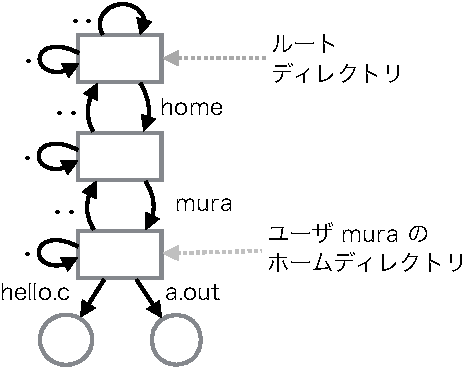
\includegraphics[scale=1.0]{Fig/FileSystem2-crop.pdf}
\end{myfig}

\subsection*{ホームディレクトリ}
ユーザがシステムにログインした時のデフォルトのカレントディレクトリを
ホームディレクトリと呼ぶ.
ホームディレクトリの位置はUNIXシステムの管理者が自由に決められる.
\figref{filesystem2}のように\texttt{/home}ディレクトリに
ユーザ名と同じ名前のディレクトリ準備し,ホームディレクトリにすることが多い
\footnote{macOSでは,\texttt{/Users} ディレクトリに作られる.}.

多くのUNIXツールではホームディレクトリのことを「\texttt{$\sim$}」と表記できる.
しかし,これはUNIXファイルシステムの機能ではない.
単にツールが内部で名前の置換えを行ってるだけである.

%----------------------------------------------------------------------------
\section{パス}
ファイル(ディレクトリも含む)は,
あるディレクトリからそのファイルへの通り道であるパス(path)により特定できる.
パスはファイル木のリンクに付いた名前を
「\texttt{/}」で区切って書いた文字列として表現する.
例えば\figref{filesystem}右下の\texttt{hello.c}ファイルは,
ルートディレクトリを起点とするパス\texttt{/home/mura/hello.c}で特定できる.
同じファイルを\texttt{/home/sige/../mura/./hello.c}でも特定できる.

\subsection*{絶対パス}
パスの先頭にある「\texttt{/}」はルートディレクリを表し,
「\texttt{/}」で始まるパスは絶対パスと呼ばれる.
絶対パスはルートディレクトリを起点にしたパスである.
上記の\texttt{/home/mura/hello.c}等は絶対パスの例である.

\subsection*{相対パス}
「\texttt{/}」以外で始めたパスは相対パスと呼ばれる.
相対パスはカレントディレクトリを起点にしたパスである.
例えばカレントディレクトリが\texttt{/home}ディレクトリの時,
\figref{filesystem}右下の\texttt{hello.c}ファイルは,
相対パス\texttt{mura/hello.c}で特定できる.
カレントディレクトリが\texttt{/home/sige}ディレクトリの時は,
相対パス\texttt{../mura/hello.c}で特定できる.

%----------------------------------------------------------------------------
\section{カレントディレクトリの変更と確認}
UNIXではプロセス(実行中のプログラム)毎にカレントディレクトリがある.
プロセスのカレントディレクトリを変更しても
他のターミナルやアプリに影響を与えないし,
次回のログインに引継がれることもない.

\subsection*{cdコマンド}
カレントディレクトリはcdコマンドで変更できる.

\begin{lstlisting}[numbers=none]
$ cd パス     # パスのディレクトリへ移動する
\end{lstlisting}

\subsection*{pwdコマンド}
カレントディレクトリのパスはpwdコマンドで確認できる.

\begin{lstlisting}[numbers=none]
$ pwd         # カレントディレクトリのパスを表示する
\end{lstlisting}

ファイルシステムが\figref{filesystem}の状態の時,
muraユーザがcd,pwdコマンドを操作した例をリスト\ref{cdpwd}に示す.
なお,muraユーザのホームディレクトリは\texttt{/home/mura}とする.

\lstinputlisting[float=btp,numbers=none,
  caption=cd,pwdコマンドの実行例,label=cdpwd]
                {Lst/cdpwd.txt}

%----------------------------------------------------------------------------
\section{リンク}
ファイルを別名(別パス)で指定できると便利なことがある.
UNIX ファイルシステムはファイルに別名を付ける方法を二つ準備している.

\subsection{ハードリンク}
これまでの例では一つのファイルに付き一つのリンクしか存在しなかったが,
本来はいくつあっても構わない\footnote{
グラフ理論の木構造とはかけ離れていくが。。。}.
このリンクのことを後に出てくるシンボリックリンクと区別するために
ハードリンクと呼ぶ\footnote{
単にリンクと呼ぶ時はハードリンクのことを指している.}.
\texttt{hello.c}ファイルに新たに二つリンクを追加した例を\figref{link}に示す.

ディレクトリは\emph{リンクを格納する特殊なファイル}である.
一つのディレクトリにいくつでもリンクを格納することができる.
また,最初から存在したリンクと後で追加したリンクの間に優劣はない.

\begin{myfig}{btp}{複数のリンクを持つファイル}{link}
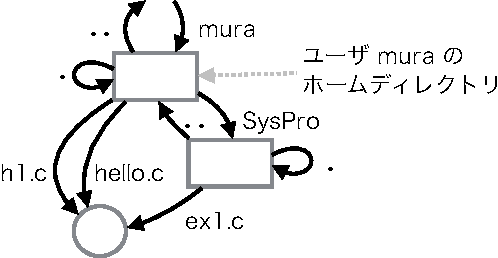
\includegraphics[scale=1.0]{Fig/Link-crop.pdf}
\end{myfig}

\subsection*{リンクの追加}
リンクの追加は次のコマンドで行う.

\begin{lstlisting}[numbers=none]
$ ln ファイルへのパス 追加するリンクのパス
\end{lstlisting}

\figref{filesystem2}の状態に二つのリンク\texttt{h1.c},\texttt{ex1.c}を追加し,
\figref{link}の状態に変える手順は次の通りである.
なお,リンク\texttt{ex1.c}を追加するより前に
\texttt{SysPro}ディレクトリを作っておく必要がある.

\lstinputlisting[numbers=none,float=ht]{Lst/ln.txt}

\subsection*{リンクの削除}

リンクの削除は rm コマンドで行う.

\begin{lstlisting}[numbers=none]
$ rm ファイルへのパス
\end{lstlisting}

rm コマンドはファイルを削除するコマンドと考えてきたが,
正確にはリンクを削除するコマンドである.
リンクを削除した結果,リンクを一つも持たなくなったファイル本体は削除される.
\emph{このようにリンクとファイル本体は別のものである.}
\figref{link}の状態から\figref{filesystem2}の状態に戻す手順を次に示す.

\lstinputlisting[numbers=none,float=ht]{Lst/lnrm.txt}

\subsection{シンボリックリンク}
シンボリックリンク\footnote{
シンボリックリンクのことをソフトリンクと呼ぶこともある.}
はパス(文字列)を格納した特殊なファイルである.
オペレーティングシステムがパスを解析する途中でシンボリックリンクを見つけると,
パス中のシンボリックリンク名をシンボリックリンクの内容で置き換えてから
パスの解析を続ける.
ハードリンクは同一の二次記憶装置内のファイルしかリンクできないが,
シンボリックリンクにはこのような制約はない.

シンボリックリンクにはどんなパスでも書き込むことができる.
まずリンク切れのシンボリックを作っておき,
後にファイル本体を作ることも許される.
一方でリンク先のファイルが削除された場合はリンク切れ状態になる.
これを応用すると,
置き換わったファイルを同じシンボリックリンクで参照し続けることができる.
\emph{リンク先ファイルが置換わることがシンボリックリンクの特徴である.}

\subsection*{シンボリックリンクの使用例}
\figref{symlink}にシンボリックリンクを使用した例を示す.
この例は\figref{link}のハードリンクをシンボリックリンクに置き換えたものである.
この図では,シンボリックリンクを内部にパスを書いた長方形で表現している.
シンボリックリンクもファイルの一種なので,
ディレクトリからハードリンクによって接続されている.

ユーザ mura のホームディレクトリからの相対パス\|h1.c|を用いてファイルを
指定した場合,パスはシンボリックリンクの内容と置き換えられ\|hello.c|になる.
同様に相対パス\|SysPro/ex1.c|は,\|ex1.c|がシンボリックリンク名なので
\|SysPro/../hello.c|に置き換えられる.
どちらの場合もホームディレクトリ直下の\texttt{hello.c}ファイルを
指定したことになる.

\begin{myfig}{btp}{シンボリックリンク}{symlink}
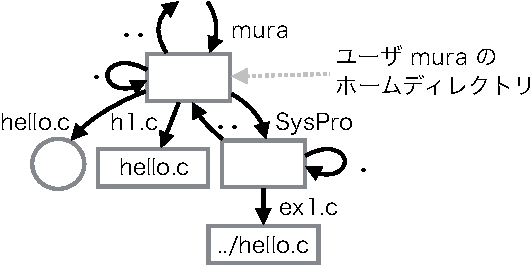
\includegraphics[scale=1.0]{Fig/SymLink-crop.pdf}
\end{myfig}

\subsection*{シンボリックリンクの作成}
シンボリックリンクは
\texttt{ln}コマンドに\texttt{-s}オプションを付けたものを用いて作成する.

\begin{lstlisting}[numbers=none]
$ ln -s リンクに書込むパス 作成するリンクのパス
\end{lstlisting}

\figref{filesystem2}の状態に
二つのシンボリックリンク\texttt{h1.c},\texttt{ex1.c}を追加し,
\figref{symlink}の状態に変える手順は次の通りである.
シンボリックリンク\texttt{ex1.c}に書込むパスは\|../hello.c|になる.
\emph{シンボリックリンクに書込むパスには
シンボリックリンクが存在するディレクトリからの相対パスを用いる\footnote{
絶対パスを書込むことも可能であるが普通は相対パスを用いる.
例えばシステム管理者がユーザ\texttt{mura}のホームディレクトリの
位置を変更しても,相対パスを用いておけばリンク切れにならない.}.}

\lstinputlisting[numbers=none]{Lst/lns.txt}

\subsection*{シンボリックリンクの削除}

シンボリックリンクの削除も\texttt{rm}コマンドで行う.

\begin{lstlisting}[numbers=none]
$ rm シンボリックリンクのパス
\end{lstlisting}

\figref{symlink}の状態から\figref{filesystem2}の状態に戻す手順を次に示す.

\lstinputlisting[numbers=none,float=ht]{Lst/lnsrm.txt}

%----------------------------------------------------------------------------
\section{ファイルの属性}
UNIXの各ファイル\footnote{ディレクトリやシンボリックリンクも含む}は,
ファイル本体にデータだけでなく幾つかの属性情報(メタデータ)を持っている.
ファイル名を属性情報の一部にしているOSも多いが,
UNIXではファイル名はファイル本体ではなくリンクに付属するので
属性に含まれていない.

\subsection{主な属性}
UNIXで用いられる主な属性情報は次の通りである.
これらは\texttt{stat}コマンドや\texttt{ls}コマンドで表示できる.

\begin{description}
\item[種類] 普通のファイル,ディレクトリ,シンボリックリンク等の区別.
\item[保護モード] openシステムコールで紹介した\texttt{rwxrwxrwx}.
\item[リンク数] ファイルを指しているハードリンクの数.
リンク数が0になるとファイル本体が削除される.
(例えば,\figref{link}の\texttt{hello.c}ファイルの場合は3になる)
\item[所有者] 所有者のユーザ番号.
\item[グループ] 属するグループのグループ番号.
\item[ファイルサイズ] ファイルの大きさ(バイト単位).
\item[最終参照日時] 最後にアクセスした時刻.
\item[最終変更日時] 内容を最後に変更した時刻.
\item[最終属性変更時刻] 属性を最後に変更した時刻.
\end{description}

\subsection{属性の表示方法}
属性を表示する専用コマンドは stat であるが,
ここでは,より手軽に使用できる ls コマンドを紹介する.
ls コマンドは\texttt{-l}オプションを付けて実行すると,
ファイルの属性情報の一部を表示する\footnote{
より多くの属性情報を知りたい時は,stat コマンドを用いる.}.
以下に ls コマンドを実行した例を示す.

\begin{lstlisting}[numbers=none]
$ ls -l a.txt
-rw-r--r--  1 mura  staff 10 May  1 18:18 a.txt
\end{lstlisting}

実行例の表示は以下の意味を持っている.

\begin{description}
\item[ファイルの種類] 一文字目の「\texttt{-}」は
ファイルが普通のファイルであることを表している.
一文字目が「\texttt{d}」はディレクトリであること,
「\texttt{l}」はシンボリックリンクであることを表す.
\item[ファイルの保護モード] openシステムコールで紹介したもの
(\texttt{rwxrwxrwx}).
\item[リンク数] \texttt{1}はリンク数が1であることを表している.
\item[所有者] \texttt{mura}は
ファイルの所有者がユーザ mura であることを表している.
メタ情報の内部表現はユーザ番号であるが,
ls コマンドがユーザ名に変換して表示している.
\item[グループ] \texttt{staff}は
ファイルがグループ staff に属することを表している.
メタ情報の内部表現はグループ番号であるが,
ls コマンドがグループ名に変換して表示している.
\item[ファイルサイズ] \texttt{10}はファイルのサイズが10バイトで
あることを表している.
\item[最終変更日時] \texttt{May 1 18:18} はファイルの最終変更日時である.
\item[パス] \texttt{a.txt} はファイルへ到達するために使用したパスである.
\emph{パス名(ファイル名)はファイルの属性ではない.}
\end{description}

\subsection{属性の変更方法}
ファイルの保護モードは一般ユーザも変更する機会が多い.
ファイルの保護モードの変更には chmod コマンドを用いる.
以下に書式を,リスト\ref{lstchmod}に使用例を示す.

\begin{lstlisting}[numbers=none]
$ chmod OOO ファイル...      # 書式1
$ chmod ugo+rwx ファイル...  # 書式2
$ chmod ugo-rwx ファイル...  # 書式3
\end{lstlisting}

\begin{description}
\item[書式1] \texttt{OOO}は3桁の8進数である.
8進数で保護モードを指定する.
8進数の値はopenシステムコールの書式2と同じである.

\item[書式2,3] \texttt{ugo+-rwx}の文字を組合せて
保護モードの変更方法を記述する.
各文字の意味は\tabref{chmod}の通りである。
例えば,
所有者とグループに書込み権と実行権を与える場合なら\texttt{ug+wx}のように書く.
その他のユーザの読出し権を取上げるなら\texttt{o-r}のように書く.
\end{description}

以下に chmod コマンドの使用例を示す.

\begin{mytable}{btp}{\texttt{chmod}コマンドの引数の意味}{chmod}
  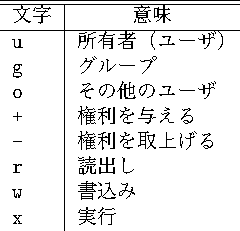
\includegraphics[scale=1.0]{Tbl/chmodOptions.pdf}
\end{mytable}

\lstinputlisting[float=btp,numbers=none,
  caption=chmodコマンドの使用例,label=lstchmod]{Lst/chmod.txt}

\newpage
\section*{課題 No.3}
以下を行い,それに用いた手順と結果を印刷して提出しなさい.

\begin{enumerate}
\item パスとハードリンク
\begin{enumerate}
\item 自分のホームディレクトリのパスを調べる.
\item ハードリンクに関する課題を行うために,
ディレクトリ\texttt{/tmp}にカレントディレクトリを移動する\footnote{
PC教室のMacは一般ユーザのホームディレクトリを共有ドライブ上に置いている.
macOSの共有ドライブ上にはハードリンクを作ることができない.
\texttt{/tmp}はローカルハードディスク上にあり,かつ,
誰でも自由に一時的なファイルを作ることができるディレクトリである.}.
\item \texttt{/tmp}以下に\figref{link}のディレクトリやファイルを作る.
\item \texttt{ls -l}を用いてファイルの種類やリンク数を確認する.
\item 相対パスを用いて\texttt{hello.c}の内容を表示する.
(表示には\texttt{cat}コマンドを用いると良い.)
\item 絶対パスを用いて\texttt{hello.c}の内容を表示する.
\item \texttt{h1.c}を利用した相対パスを用いて\texttt{hello.c}の内容を表示する.
\item \texttt{ex1.c}を利用した相対パスを用いて
\texttt{hello.c}の内容を表示する.
\item カレントディレクトリを\texttt{SysPro}に変更する.
\item \texttt{ex1.c}を利用した相対パスを用いて
\texttt{hello.c}の内容を表示する.
\item \texttt{hello.c}を利用した相対パスを用いて
\texttt{hello.c}の内容を表示する.
\item ディレクトリのハードリンクができるか試す.
\item 課題のために作成したファイルやディレクトリを全て削除する.
\end{enumerate}

\item シンボリックリンク
\begin{enumerate}
\item シンボリックリンクを作ってみる.
\item シンボリックリンクを\texttt{ls -l}を用いて確認する.
\item シンボリックリンクを用いてファイルをアクセスできることを確認する.
\item リンク切れのシンボリックリンクを使用するとどうなるか確認する.
\item ディレクトリに対するリンクを作って使用できることを確認する.
\item 他のディレクトリにあるファイルをリンクして使用できることを確認する.
\item シンボリックリンクのループを作る.(a.txt →  b.txt,b.txt →  a.txt)
\item ループしているシンボリックリンクを使用するとどうなるか確認する.
(\|$ cat a.txt|)
\end{enumerate}

\item 保護モード
\begin{enumerate}
\item テキストファイル(\texttt{hello.c})と
実行可能ファイル(\texttt{a.out})を準備する.
\item \texttt{chmod}で保護モードを変化させてみる.
\item \texttt{ls -l}で変化を確認する.
\item 保護モードを変化させて,ファイルの読出しや実行ができるか確認する.
\item ディレクトリの保護モードは何の意味を持つか考える.
\end{enumerate}
\end{enumerate}
